\documentclass[a4paper, 12pt, twoside]{report}
\usepackage{natbib}
\renewcommand{\bibpreamble}{\vskip1cm}
\usepackage[nottoc,notlot,notlof]{tocbibind}

\usepackage{tocloft}
\renewcommand{\contentsname}{\makebox[\linewidth]{Table of Contents}}
\renewcommand{\cfttoctitlefont}{\normalsize\bfseries}

\renewcommand{\cftloftitlefont}{\hspace*{\fill}\normalsize\bfseries}
\renewcommand{\cftafterloftitle}{\hspace*{\fill}}

\renewcommand{\cftlottitlefont}{\hspace*{\fill}\normalsize\bfseries}
\renewcommand{\cftafterlottitle}{\hspace*{\fill}}

\renewcommand\cftchapfont{\mdseries}
\renewcommand\cftchappagefont{\mdseries}

\setlength{\cftbeforetoctitleskip}{-2.4em}
\setlength{\cftbeforeloftitleskip}{-2.4em}
\setlength{\cftbeforelottitleskip}{-2.4em}
\addtocontents{toc}{\vspace{-3em}}
\addtocontents{lof}{\vspace{-3em}}
\addtocontents{lot}{\vspace{-3em}}

\usepackage{titlesec}
\titleformat{\chapter}[block]{\bfseries}{\chaptertitlename\ \thechapter}{1em}{}
\titlespacing*{\chapter}{0pt}{-29.3pt}{10pt}
\titleformat{\section}[block]{\bfseries}{\thesection }{1em}{} 
\titlespacing*{\section}{0pt}{20pt}{5pt}
\titleformat{\subsection}[block]{\bfseries}{\thesubsection }{1em}{}
\titlespacing*{\subsection}{0pt}{10pt}{5pt}

\usepackage{blindtext}
\usepackage[utf8]{inputenc}
\usepackage[top=2.36cm, bottom=2.5cm, outer=2.5cm, inner=4cm]{geometry}
\usepackage{setspace}
\setstretch{2}
\usepackage{newtxtext,newtxmath}

\usepackage{times}
\usepackage{soul}
\usepackage{url}
\usepackage[hidelinks]{hyperref}
\usepackage{graphicx}
\usepackage{amsmath}
\usepackage{booktabs}
\usepackage{algorithm}
\usepackage{algorithmic}
\usepackage[caption=false]{subfig}

\usepackage{color,soul}
\usepackage{amsmath, amssymb, bm}
\usepackage{multirow}
\usepackage{bigstrut}
\usepackage{resizegather}
\usepackage{array}

\usepackage{booktabs}
\usepackage{mwe}
\usepackage{longtable}
\usepackage{lineno,hyperref}

\usepackage{chngcntr}
\counterwithin{figure}{section}
\counterwithin{table}{section}

\usepackage{enumitem}

\usepackage{calc}

\setlength{\cftsecindent}{0pt}
\setlength{\cftsubsecindent}{28pt}
\renewcommand{\cftchappresnum}{Chapter }
\AtBeginDocument{\addtolength\cftchapnumwidth{\widthof{\bfseries Chapter }}}
\renewcommand{\cftchapleader}{\cftdotfill{\cftdotsep}}

\setlength{\cftfigindent}{0pt}  % remove indentation from figures in lof
\setlength{\cfttabindent}{0pt}  % remove indentation from tables in lot

\usepackage{lipsum}

\title{}
\author{}
\date{}

\let\cleardoublepage=\clearpage

\begin{document}
\newgeometry{top=2.54cm, bottom=2.54cm, left=3.18cm, right=3.18cm}
\begin{titlepage}
    \begin{center}
        \vspace*{2.5cm}
         \large
        The Latex Template of UM Doctoral Thesis
 
        \vspace{0.8cm}
        \large
        by
 
        \vspace{0.8cm}
 
        Bo Liu
 
        \vspace{0.8cm}
 
        Doctor of Philosophy in Computer Science
        
        \vspace{0.5cm}
        
        %(Draft)
 
        \vspace{4cm}
        
        2020
        
        \vspace{1cm}
 
        
\includegraphics[width=0.3\textwidth]{university}
        
        %\vspace{0.5cm}
 
        \large
        Faculty of Science and Technology\\
        University of Macau\\
        
 
    \end{center}
\end{titlepage}

\begin{titlepage}
    \begin{center}
        \vspace*{1.5cm}
        \large
 
        
        The Latex Template of UM Doctoral Thesis 
        
        \vspace{1.2cm}
 
        by
 
        \vspace{1.2cm}
 
        Bo Liu
 
        \vspace{1.2cm}
 
        SUPERVISOR: Prof. Chi-Man Pun
 
        \vspace{1.2cm}
        
        DEPARTMENT: Department of Computer and Information Science
        
        \vspace{1.2cm}
 
        Doctor of Philosophy in Computer Science
        
        \vspace{1.2cm}
 
        2020
        
        \vspace{1.2cm}
        
        Faculty of Science and Technology
        
        \vspace{1.2cm}
        
        University of Macau

    \end{center}
\end{titlepage}

\begin{titlepage}
    \begin{center}
        \vspace*{6.23cm}
        \large
 
       Author's right 2020 by\\
       LIU, Bo
 

    \end{center}
\end{titlepage}

\restoregeometry
\pagenumbering{roman}

\chapter*{\makebox[\linewidth]{Acknowledgements}}
\addcontentsline{toc}{chapter}{Acknowledgements}
%write your acknowledgements here and delete lipsum[1] and lipsum[2]
\lipsum[1]
\\

\noindent
\lipsum[2] 

\chapter*{\makebox[\linewidth]{Abstract}}
\addcontentsline{toc}{chapter}{Abstract}
%write your abstract here and delete limpsum [1]~[4]
\lipsum[1]

\lipsum[2]

\lipsum[3]

\lipsum[4]

\chapter*{\makebox[\linewidth]{Declaration}}
\addcontentsline{toc}{chapter}{Declaration}
I declare that the thesis here submitted is original except for the source materials explicitly acknowledged and that this thesis as a whole, or any part of this thesis has not been previously submitted for the same degree or for a different degree.\\

\noindent
I also acknowledge that I have read and understood the Rules on Handling Student Academic Dishonesty and the Regulations of the Student Discipline of the University of Macau.

\newpage

\tableofcontents

\cleardoublepage
\addcontentsline{toc}{chapter}{\listfigurename}
\listoffigures
\newpage
\cleardoublepage
\addcontentsline{toc}{chapter}{\listtablename}
\listoftables


\newlist{abbrv}{itemize}{1}
\setlist[abbrv,1]{label=,labelwidth=1in,align=parleft,itemsep=0.4\baselineskip,leftmargin=!}
\chapter*{\makebox[\linewidth]{List of Abbreviations}}
\addcontentsline{toc}{chapter}{List of Abbreviations}
\chaptermark{List of Abbreviations}
\begin{abbrv}
\item[CRF]			Conditional Random Field
\item[FCN]          Fully Convolutional Network
\item[CNN]          Convolutional Neural Network
\item[SVD]          Singular Value Decomposition 
\item[SVM]          Support Vector Machine
\item[CFA]          Color Filter Array
\item[PRNU]         Photo Response Non-uniformity
\item[NLF]          Noise Level Function

\end{abbrv}

\maketitle
%This command will generate a blank page. When you bind the printed manuscript, please remove this blank page.
%But do not delete this command, otherwise it will cause problems. So just remove it from printed thesis. 

\pagenumbering{arabic}
\chapter{Introduction}
\section{General Background}
Intentionally manipulation of photos has a long history, and in most cases, forged pictures are only used to entertain the public without harms. With the development of computer hardware and software, creating a fake picture, compositing two people kissing each other for example, is easy to implement even for untrained ordinary people. However, pictures as photography for significant events, news report, and judicial evidence must be proven to be authentic. Misinformation and fake news propagate rapidly on the Internet, and they will mislead the public because people always tend to trust their eyes. An effective and efficient image forensic tool is therefore strongly needed in practical use. There are three categories of commonly seen image manipulations: copy-move forgery attempting to copy an object and then paste to a different location in the same image; photo inpainting removing something unwanted in an image and filling the position with its background; splicing forgery adding an image with visual elements from other pictures. In this thesis, we focus on the third manipulation. 

Active \cite{RN56, RN55} and blind authentication methods \cite{is1, is2} are two categories to detect splicing forgery. Because most existing pictures are source unknown but non-blind methods require operation on source images, blind detection methods show more flexibility and feasibility. To discriminate whether a picture has undergone digital splicing, the technique of watermarking can be used \cite{RN59}. If the watermarking of the picture changes, the picture is regarded as being altered in some ways such as copy-move forgery or splicing forgery. But those methods require the original pictures to produce the watermark, thus given a test picture without any watermark they cannot make a judgment. Moreover, producing watermarks for every picture taken by cameras is impossible. Therefore, there is a strong need for methods which can detect forgery without a prior.

\section{Research Goals and Objectives}
Methods based on noise difference tend to locate spliced areas by threshold \cite{Lyu}. Those areas with noise discrepancy over a pre-set threshold will be marked. Though performing good in estimating global noise variance of a given image, prior works are not designed for dealing with small areas, thus improper for splicing detection. Besides, the problem of noise fluctuation is not well solved, resulting in higher false positive ratios, which significantly interrupts the observer's judgment. The first goal of this work is to address two issues by adaptive-SVD noise estimation for small area and SVM for noise fluctuation.

\section{Research Methodology and Design}
Four methods are designed to accomplish the research goals and objectives in this thesis. These methods are under the framework of supervised learning, with one method adopting SVM as the classifier and three algorithms using deep neural networks.

Base on the fact that images from different origins should have a different amount of noise produced by image sensors or post-processing by software, I proposed a novel detection method by analyzing noise discrepancy to expose and locate splicing forgery in digital images. To improve the accuracy of noise estimation, I proposed the Adaptive Singular Value Decomposition (Adaptive-SVD) to estimate the local noise. By combining local and global noise clues, I proposed the Vicinity Noise Descriptor to locate splicing forgery. Regional forensic information is inferred via machine learning method - Support Vector Machine (SVM). To evaluate the proposed method, I constructed splicing forgery databases which include various scenarios and different spliced objects with artificially added or camera-generated noise. 

\section{Potential Contributions}
In the first proposed method, the contributions include 1)The proposed adaptive Singular Value Decomposition improves the accuracy of noise estimation in small area, meanwhile, to decompose the image into several levels in which the noise level of each region bears comparability. The multi-level analysis in return improves the accuracy of noise estimation as well. The method solves the problem that the estimation becomes unreliable when the image segment is small in previous study \cite{RN54}, which demonstrates noise estimation of the whole image based on Singular Value Decomposition outperforms existing methods in terms of accuracy. 2)To handle noise fluctuating among regions, I proposed vicinity noise descriptor and adopted supervised learning framework - support vector machine to learn from our created training database, which contains original and spliced pictures, and then to locate spliced areas in real test, resulting significantly lower false positive ratio of detection.

\section{Organization of the Thesis}
This chapter gives the general background of the problem of blind splicing forgery detection, and the research goals and objectives are also presented. Research methodology and design, as well as the contributions of the work are described in the chapter. The remaining part of the thesis is organized as follows. 

In chapter 2, the related work of this thesis are described in detail. 

The first algorithm with adaptive-SVD noise estimation and SVM as a classifier together with experimental results will be introduced in chapter 3. 

Chapter 4 discusses the method with the deep learning framework where CNN and FCN are combined to make predictions. Relevant experiments are also presented.

In chapter 5 and chapter 6, two deep fusion networks will be introduced in detail. The first fusion network in chapter 5 is a fusion of different networks while the latter in chapter 6 is a single network takes fusion data which implements different hypotheses of forgeries. Experiments and comparisons to state-of-the-arts are also included. 

Chapter 7 concludes the thesis and states the limitations of the proposed algorithms, and gives the future works. 

\section{Statement of Originality}
I declare that the work presented in this thesis is, to the best of my knowledge and belief, original, except as acknowledged in the text. And the results have not been submitted for a degree at this or any university. The work was done under the guidance of my supervisor, Professor Chi-Man Pun.

\textbf{\textit{Publications}}
\begin{enumerate}
    \item Liu, Bo, and Chi-Man Pun. "Thesis Template" \textit{Journal of University of Macau} 526 (2020):133-150.
    \item Liu, Bo, and Chi-Man Pun. "Graduation Soon" \textit{Happy Journal of Ph.D.} 387 (2020): 172-187.
\end{enumerate}

\chapter{Related Work}
\lipsum[1]

\section{Detecting splicing forgery by noise discrepancy}
\lipsum[1]

\lipsum[2]

\section{Detecting splicing forgery by JPEG compression traces}
\lipsum[1]

\section{Detection splicing forgery by deep learning without priors}
\lipsum[2]

\section{Fusion of hypotheses to expose splicing forgery}
\lipsum[3]

\chapter{Adaptive-SVD Noise Estimation and Vicinity Noise Descriptor for Locating Splicing}\label{s2}
Liu and Lin \cite{RN54} estimate the additive noise in image by uncovering linear relation between average of tail singular values ${{P}_{M}}$ and noise variance $\sigma $. And this correlation is an important preliminary condition in their analysis.  Fig. \ref{tip13c} shows this correlation under different image sizes. The linear correlation is obvious when the image size is large, for example, $256\times 256$, while in the small sized $16\times 16$ and $32\times 32$ images, it is unstable. However, in detection of splicing forgery, the image segments are unavoidably small for better splicing locating. Therefore, we proposed adaptive-SVD to improve the estimation accuracy in small image segments. 
\begin{figure}[!htbp]
	\centering
	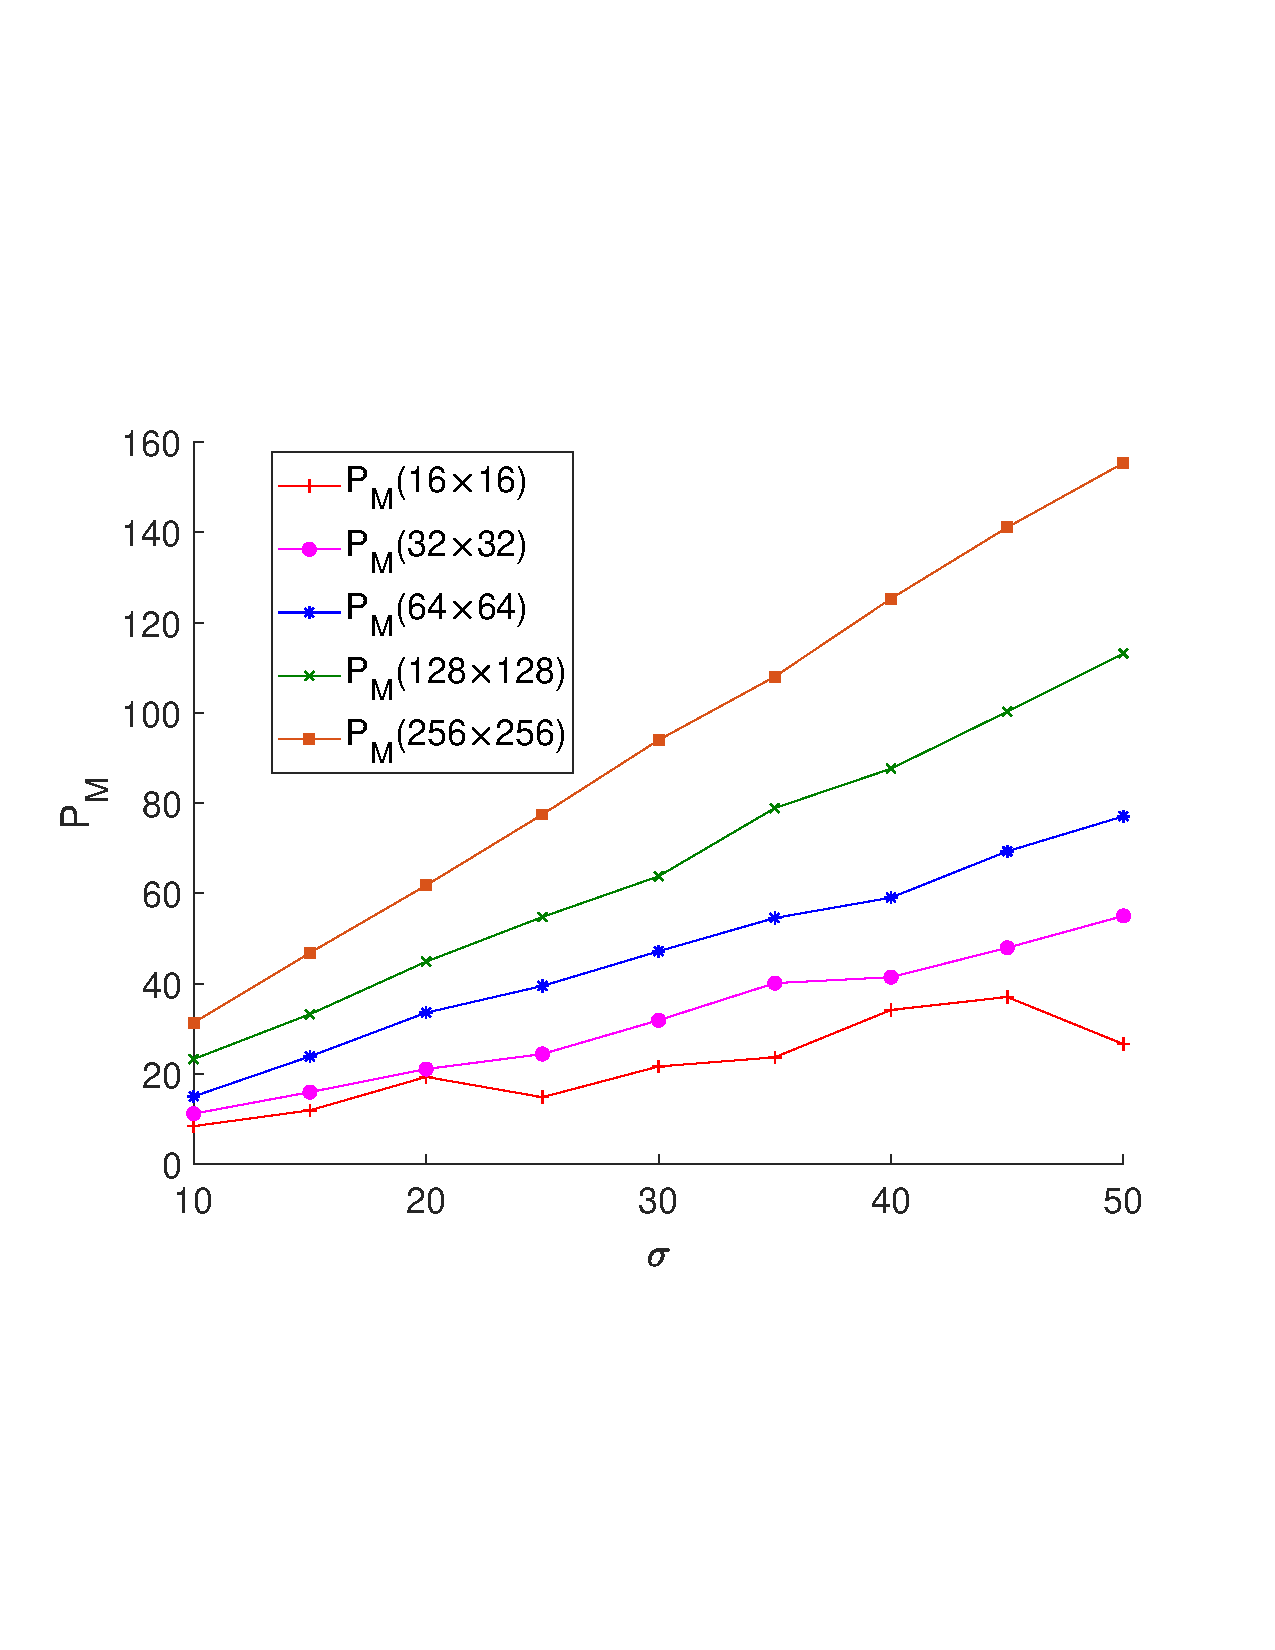
\includegraphics[width=0.8\textwidth]{tip13c}
	\caption{Noise variance and average of tail singular values in different sized images.}
	\label{tip13c}
\end{figure}

\section{Adaptive-SVD noise estimation}\label{s2a}
The singular value relates to the noise in image, thus can be used for noise estimation and denoising\cite{RN136}. Liu \cite{RN54} models linear dependency between the noise variance of image and its tail singular values. Their method performs well when pictures are in normal or large size. However, when the image size is small, the detection accuracy falls. Therefore, it is not feasible to apply this method directly to splicing detection, in which image segments are small. Since tail singular values, rather than initial ones, relate to the noise signal, we can set initial singular values to zeros to filter out most part of the image, leaving noise signal for analysis. Changing column vectors in left orthogonal matrix gets equivalent result.

Formally, given $m\times n$ image matrix $A$, the singular value decomposition can be denoted by
\begin{equation}
	A=U\times S\times {{V}^{T}}
\end{equation}
where $U$ is a $m\times m$ orthogonal matrix, $S$ is a $m\times n$ diagonal matrix containing singular values and ${{V}^{T}}$ is the transposition of  another $n\times n$ orthogonal matrix. Suppose $r$ is the rank of matrix $A$ and we expand $U$ as \[U=({{u}_{1}},{{u}_{2}},...,{{u}_{m}})\]and denote singular values in $S$ as $s(i),i=1,2,...,r$ , and evidently $s(1)>s(2)>...>s(r)$. 

Set initial column vectors ${{u}_{1}},{{u}_{2}},...,{{u}_{k}},1<k<m$ to 0, the modified $U$ denoted by ${{U}_{k}}=(0,0,...0,{{u}_{k+1}},{{u}_{k+2}},...{{u}_{m}})$ and then reconstruct the original image matrix ${{\tilde{A}}_{k}}$ by 
\begin{equation}
	{{\tilde{A}}_{k}}={{U}_{k}}\times S\times {{V}^{T}}
	\label{svdequation}
\end{equation}

Reconstructed matrix ${{\tilde{A}}_{k}}$ contains noise signal mostly and its variance ${{\sigma }_{{\tilde{A}}}^{2}}$ is regarded as estimated noise variance $\tilde{\sigma }_{A}^{2}$ approximately. Formally,
\begin{equation}
	\left. \tilde{\sigma }_{A}^{2} \right|k=\sigma _{{\tilde{A}}}^{2}=\frac{1}{n}\sum{{{({{a}_{ij}}-\bar{a})}^{2}}}
\end{equation}

$\left. \tilde{\sigma }_{A}^{2} \right|k$ is estimated noise variance for image matrix $A$ when initial $k$ column vectors of $U$ are set to 0; ${{a}_{ij}}$ is the element of matrix and $\bar{a}$ is average value of all elements in reconstructed matrix ${{\tilde{A}}_{k}}$. Given a $m\times n$  image matrix, there are $m-2$ values that $k$ can be set. We will introduce an adaptive algorithm to determine the proper value of $k$. And this process will simultaneously produce multi-level noise maps for splicing detection.

For a random variable $X$ with mean value of $\mu $ and  variance of ${{\sigma }^{2}}$, the skewness and kurtosis is defined as
\begin{equation}
	skew(X)=\frac{\mathbb{E}[{{(X-\mu )}^{3}}]}{{{({{\sigma }^{2}})}^{3/2\;}}} 
\end{equation}
\begin{equation}
	kurt(X)=\frac{\mathbb{E}[{{(X-\mu )}^{4}}]}{{{({{\sigma }^{2}})}^{2}}}-3
\end{equation}
where $\mathbb{E}[\cdot ]$ is mathematical expectation. For Gaussian distribution, the value of skewness and kurtosis equals to 0. Since the noise in the image is assumed to be Gaussian distributed, the value of skewness and kurtosis of reconstructed image matrix ${{\tilde{A}}_{k}}$ is expected to approximate to 0 if it contains noise signals mostly. We can therefore find this ideal matrix from the set $\left\{ \left. {{{\tilde{A}}}_{k}} \right|1<k<m \right\}$ by comparing the skewness of each matrix in the set. 4. Both the skewness and the kurtosis can be used to determine the optimal value of k, and in the experiment, they show an equal performance. Therefore, I used the skewness to perform the selection.The reconstructed matrix with the skewness closest to 0 is regarded as the best candidate for noise estimation. Because ${{\tilde{A}}_{k}}$ is determined by $k$, we get the optimal value of $k$ by Equation \ref{bestk} and then we get ideal approximating matrix ${{\tilde{A}}_{{\hat{k}}}}$. 
\begin{equation}
	\hat{k}=\arg \underset{k}{\mathop{\min }}\,\left| skew({{{\tilde{A}}}_{k}}) \right|
	\label{bestk}
\end{equation}

Consequently the noise variance of image matrix $A$ can be estimated directly from reconstructed matrix ${{\tilde{A}}_{{\hat{k}}}}$ by Equation \ref{svdequation}. 

It is evident that for a reconstructed image matrix ${{\tilde{A}}_{k}}$, the value of estimated noise variance is tend to be smaller as the value of $k$ increases. This is because the bigger $k$ will erase more signal which includes both the image content and the noise, although the filtered image content is more than noise. Fig. \ref{svd} illustrates this phenomenon: the $23\times 23$ image segment is decomposed: the head and tail 5 singular values will be initially set to 0. Then the skewness and variance of the reconstructed matrices are computed under different $k$. Optimal estimation appears at $k=10$ and denoted by red dot. 

\begin{figure}[!htbp]
	\centering
	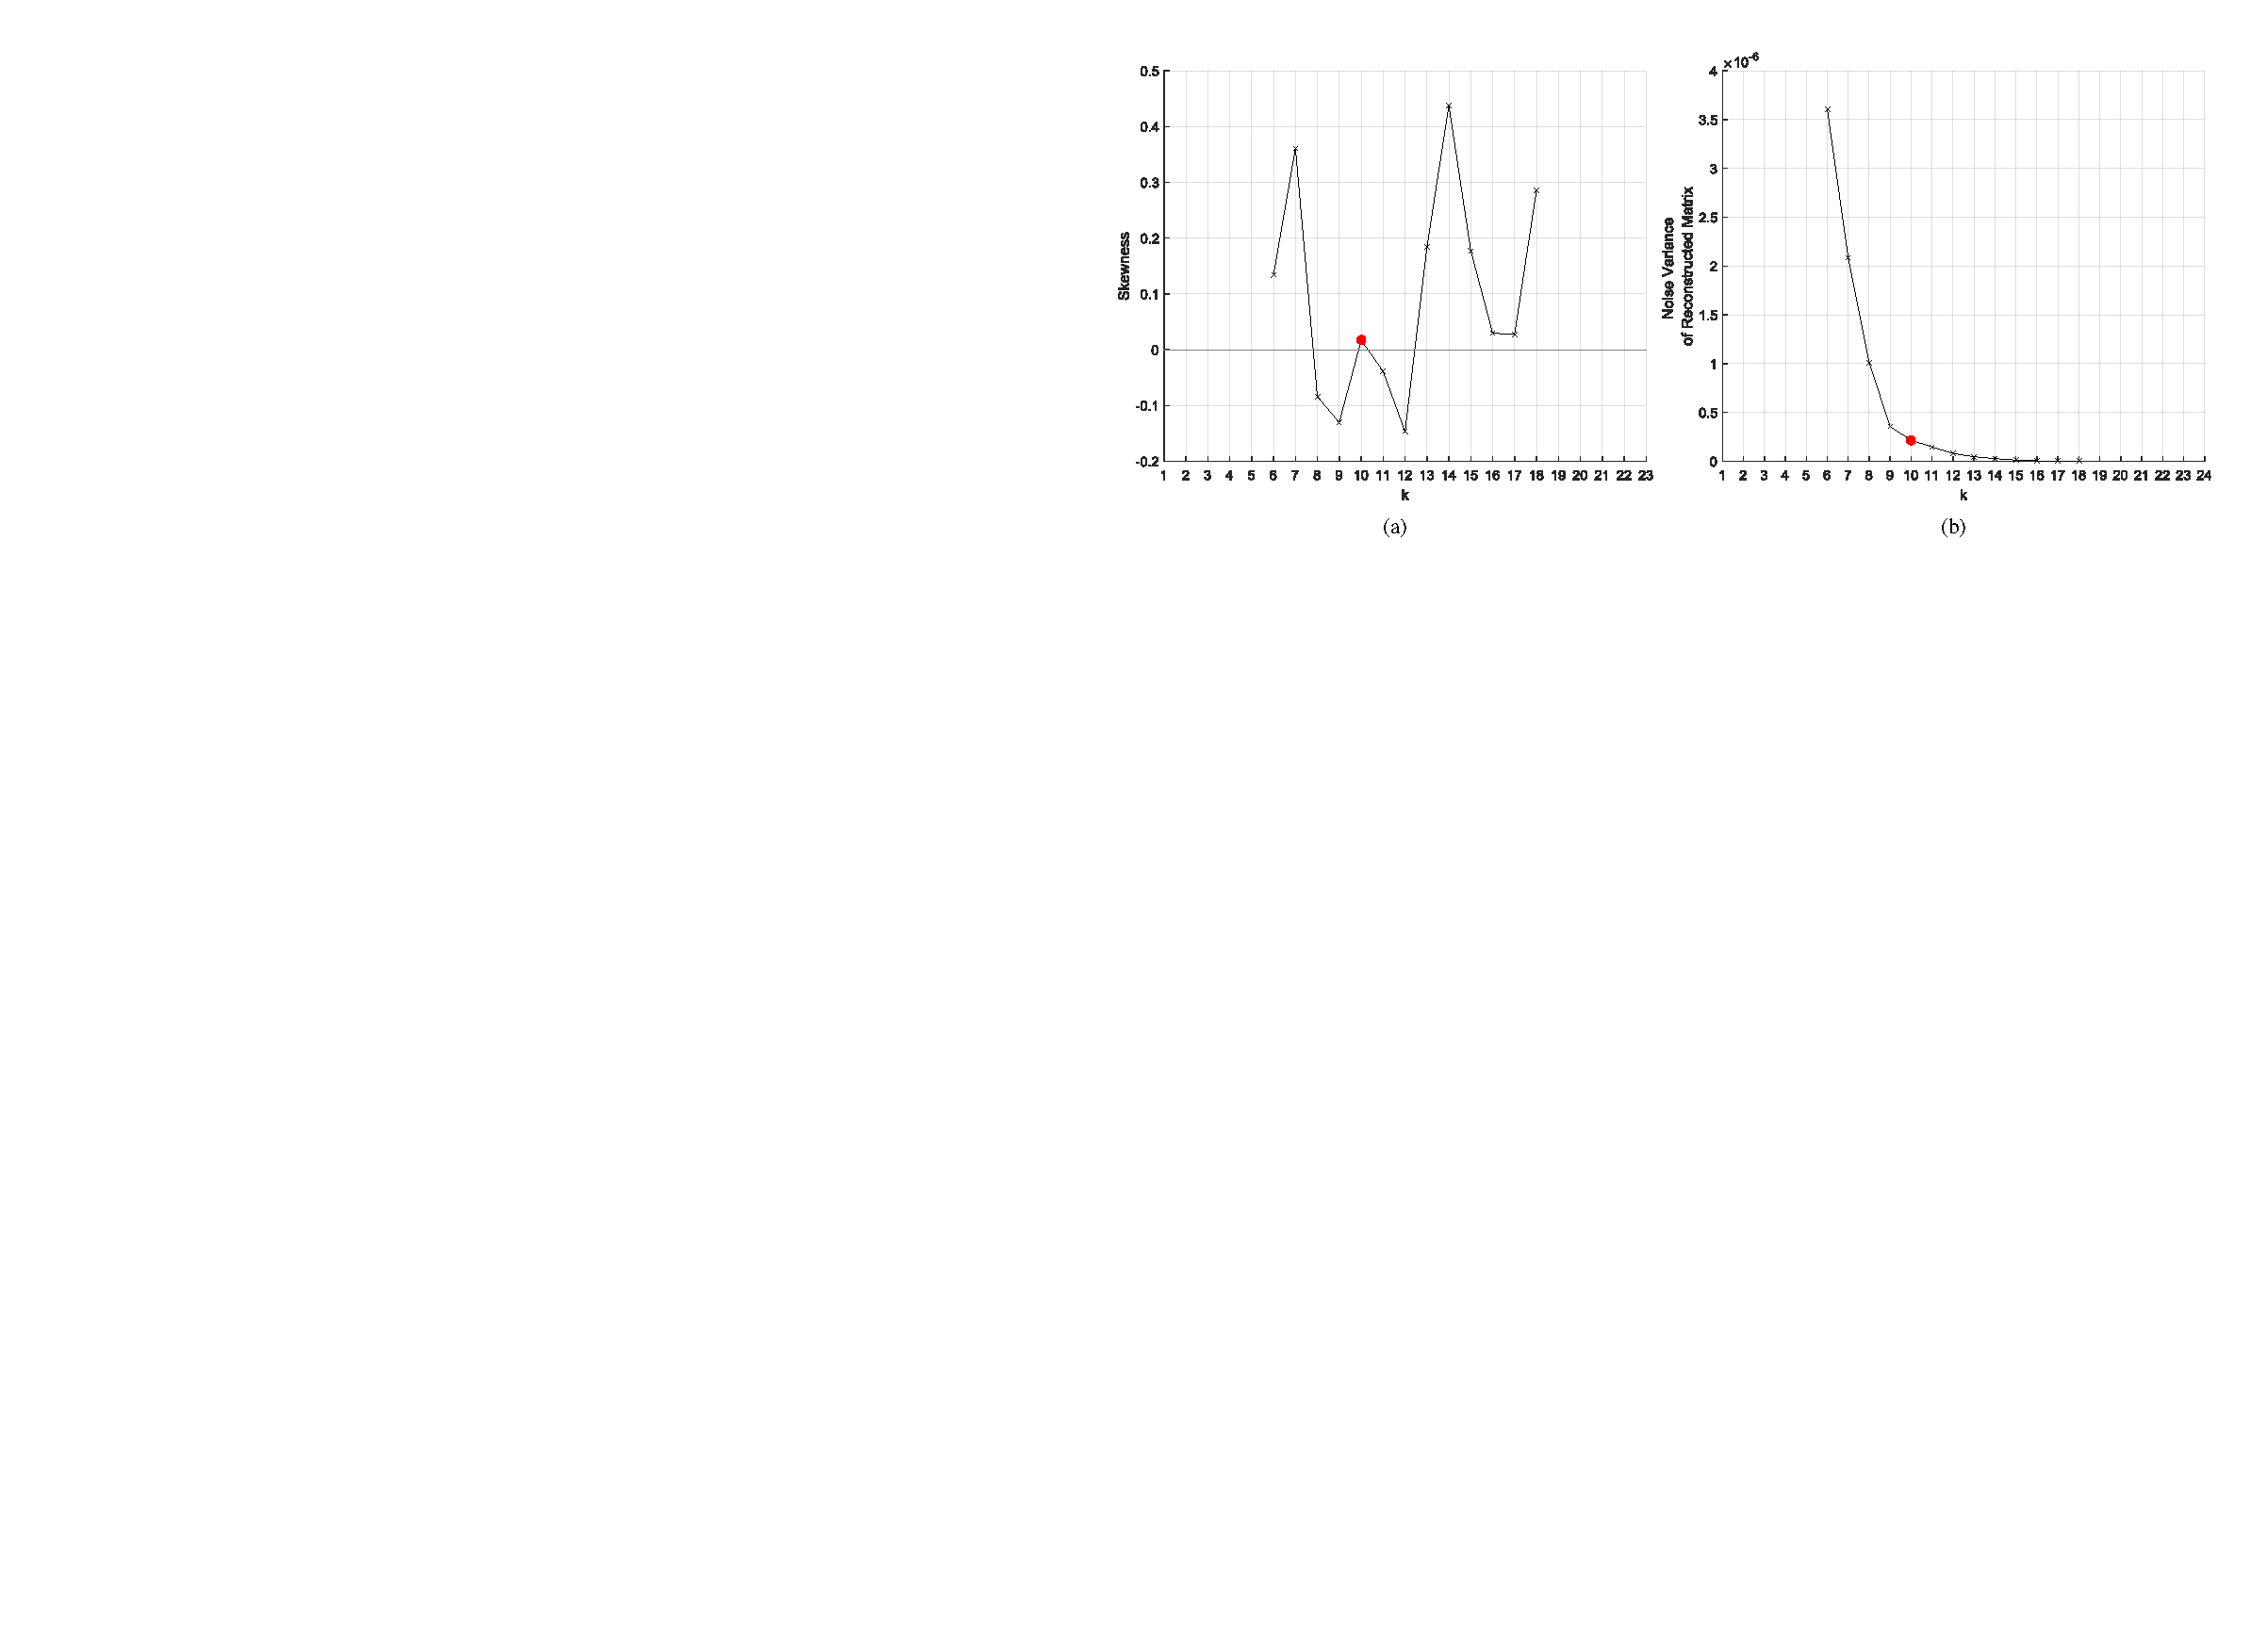
\includegraphics[width=\textwidth]{svdv3.pdf}
	\caption{Noise estimation of $23\times 23$ image segment. (a) Skewness of each reconstructed matrix under different $k$. (b) Estimated noise variance of each matrix.}
	\label{svd}
\end{figure}

Though our estimation scheme gives the optimal approximation towards the noise signal, this damping effect leads to unwanted result in splicing detection. Therefore, we introduce the multi-level noise maps to reduce the side effect of this phenomenon. For several same size $m\times m$ image matrices from a single image $I$ : $\{{{A}^{1}},{{A}^{2}},...,{{A}^{p}}\}\subset I$, where $p$ is the total number of image matrices divided from the single image $I$. The optimal reconstructed matrix for each original image matrix is $\tilde{A}_{{{{\hat{k}}}_{1}}}^{1},\tilde{A}_{{{{\hat{k}}}_{2}}}^{2},...,\tilde{A}_{{{{\hat{k}}}_{p}}}^{p},1<{{\hat{k}}_{1}},{{\hat{k}}_{2}},...,{{\hat{k}}_{p}}<m$ respectively. The interval $(1,m)$ is divided into $s$ length equal sub-intervals $(1,m/s],(m/s,2m/s],...,(m-m/s,m)$, and each $\hat{k}$ will fall into one sub-interval. Replacing the longer interval $(1,m)$ with shorter sub-intervals reduces the damping effect, making estimated noise variance from the reconstructed matrix in the same sub-interval comparable. Consequently these estimated noise variance in the same sub-interval compose a noise map and we name it noise map $M$ in level $i$ , denoted by ${{M}_{i}},1\le i\le s$. A noise map $M_i$ is composed of the estimated noise variances of certain image matrices $\tilde{A}_{\hat{k}_p}^p$. The $\hat{k}$ number of these image matrices are from the same sub-intervals $(1,m/s]$ or $(m/s,2m/s]$ or $,...,(m-m/s,m)$. Since there are s sub-intervals in total, the algorithm will produce $s$ noise maps $M_i, 1 \le i \le s$ consequently.

We have introduced how to properly estimate the noise variance of a given image matrix via adaptive-SVD. It is necessary to make clear how to produce image matrices from a single image as the first step in our proposed method. Traditionally, the image is divided into either overlapped or non-overlapped blocks for further processing. Using overlapped blocks shows better accuracy but it is time consuming, while processing non-overlapped blocks is time efficient but the performance falls. We want to locate the spliced regions preciously but those two dividing approaches cannot trace the boundaries of objects. Therefore, we proposed a new method to produce image matrices effectively and efficiently by combining SLIC Superpixels and non-overlapped method.

\begin{figure}[!htbp]
	\centering
	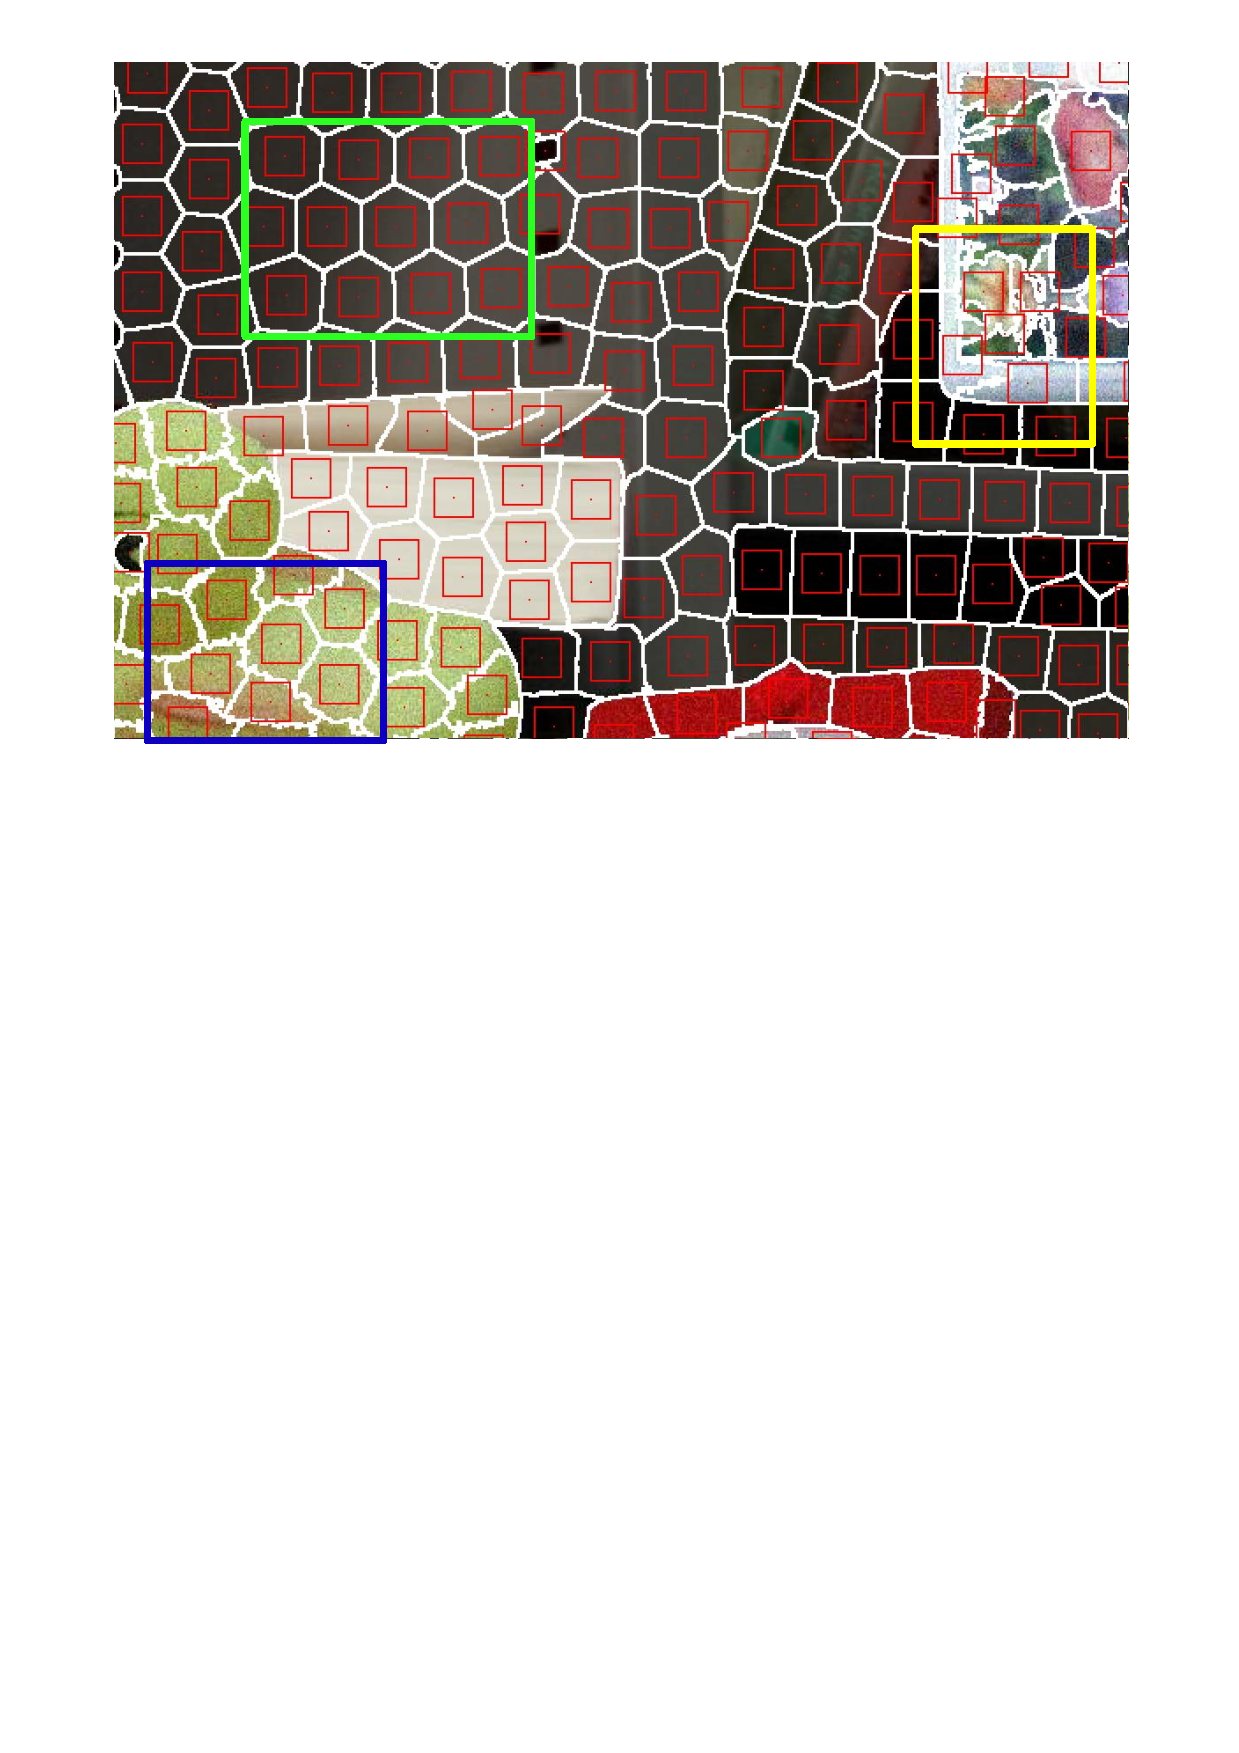
\includegraphics[width=3in]{RegularSegment.pdf}
	\caption{Obtaining image matrices for noise estimation. White cells are SLIC segments and red squares are matrices for noise estimation.}
	\label{segment}
\end{figure}

SLIC Superpixels efficiently generates compact and almost uniform superpixels while preserving boundaries \cite{RN80}. Therefore, it is utilized as the first step to segment the whole image $I$ into small segments ${{S}_{1}},{{S}_{2}},...,{{S}_{n}}$. And then in each irregular segment ${{S}_{i}},1<i<n$ , the geometrical center ${{C}_{i}}$ is computed. Regular $m\times m$ image matrix ${{A}_{i}}$ centered at ${{C}_{i}}$ is then performed adaptive-SVD noise estimation. Fig. \ref{segment} shows our segmentation scheme: the white irregular cells are results from SLIC segmentation while red squares centered at geometric center of each segments are used for noise estimation. Squares in the green box are regularly placed like non-overlapped dividing because that area is smooth. Squares in blue box are well placed in the object. Some squares in yellow box are discarded because their SLIC segmentation results are too small to obtain appropriate window for noise estimation. The estimated noise variance of  matrix ${{A}_{i}}$ will be regarded as noise variance of segment ${{S}_{i}}$ . At this point, the whole process to generate multi-level noise maps from an image has been presented.

\section{Vicinity Noise Descriptor for Splicing Inference}\label{s2b}
\lipsum[1]

\lipsum[2]

\section{Experimental Results and Discussions}\label{s3}
The sub-chapter begins with the introduction of our created forgery datasets, followed by the evaluation of our proposed Adaptive-SVD noise estimation algorithm, and we compared it with the method that noise residual was obtained by noise reduction where state-of-the-art noise reduction algorithm BM3D was used. To demonstrate the robustness of our method against other types of noise, we also tested it on a tampered image dataset where spliced area was corrupted by Poisson Noise or Pepper and Salt Noise. Then SVM training process was performed on training dataset we created, and experimental results obtained from testing dataset were compared with existing methods. In the last sub-chapter, we performed evaluation under a more realistic situation: the tampered image was composed of pictures taken with different ISO settings, and no noise was artificially added to the spliced area.

\subsection{Forgery Datasets}
\lipsum[1]

The testing dataset includes 35 subsets, covering various splicing scenarios in the real. The Table \ref{svd_tab1} shows detailed information of each subset.Note that injected area was not undergone any geometrical or color changes. Photos in subset \#1$\sim$\#5 contains exact one spliced object, covering about only 5\% area of the image frame. While this ratio rises to over 20\% in subset \#31$\sim$\#35. We also added very small amount of noise in some datasets, like \#1, \#6 and so on, in order to simulate extreme situations. The training datasets were created in a similar way, and it will be explained in later part.

\begin{table}[htbp]
\renewcommand\arraystretch{0.65}
	\centering
	\caption{Specification of Testing Dataset}
	\scalebox{0.8}[0.75]{\begin{tabular}{m{0.1\columnwidth}<{\centering}m{0.1\columnwidth}<{\centering}m{0.2\columnwidth}<{\centering}m{0.2\columnwidth}<{\centering}m{0.15\columnwidth}<{\centering}}
		\hline
		Subset \# & Number of Images & Number of Spliced Objects & Average Proportion of Spliced Region Size & Added Gaussian Noise (Variance) \bigstrut\\
		\hline
		\#1   & 49    & \multirow{5}[10]{*}{1 object} & 4.73\% & 0.001 \bigstrut\\
		\cline{1-2}\cline{4-5}    \#2   & 40    &       & 4.43\% & 0.003 \bigstrut\\
		\cline{1-2}\cline{4-5}    \#3   & 45    &       & 5.13\% & 0.005 \bigstrut\\
		\cline{1-2}\cline{4-5}    \#4   & 45    &       & 4.31\% & 0.007 \bigstrut\\
		\cline{1-2}\cline{4-5}    \#5   & 49    &       & 5.00\% & 0.01 \bigstrut\\
		\hline
		\#6   & 47    & \multirow{5}[10]{*}{2 objects} & 10.20\% & 0.001 \bigstrut\\
		\cline{1-2}\cline{4-5}    \#7   & 45    &       & 7.95\% & 0.003 \bigstrut\\
		\cline{1-2}\cline{4-5}    \#8   & 44    &       & 8.32\% & 0.005 \bigstrut\\
		\cline{1-2}\cline{4-5}    \#9   & 45    &       & 9.51\% & 0.007 \bigstrut\\
		\cline{1-2}\cline{4-5}    \#10  & 42    &       & 10.48\% & 0.01 \bigstrut\\
		\hline
		\#11  & 44    & \multirow{5}[10]{*}{3 objects} & 13.05\% & 0.001 \bigstrut\\
		\cline{1-2}\cline{4-5}    \#12  & 44    &       & 12.97\% & 0.003 \bigstrut\\
		\cline{1-2}\cline{4-5}    \#13  & 49    &       & 13.80\% & 0.005 \bigstrut\\
		\cline{1-2}\cline{4-5}    \#14  & 49    &       & 12.84\% & 0.007 \bigstrut\\
		\cline{1-2}\cline{4-5}    \#15  & 47    &       & 14.06\% & 0.01 \bigstrut\\
		\hline
		\#16  & 46    & \multirow{5}[10]{*}{4 objects} & 17.23\% & 0.001 \bigstrut\\
		\cline{1-2}\cline{4-5}    \#17  & 45    &       & 16.08\% & 0.003 \bigstrut\\
		\cline{1-2}\cline{4-5}    \#18  & 51    &       & 17.77\% & 0.005 \bigstrut\\
		\cline{1-2}\cline{4-5}    \#19  & 42    &       & 18.30\% & 0.007 \bigstrut\\
		\cline{1-2}\cline{4-5}    \#20  & 42    &       & 16.42\% & 0.01 \bigstrut\\
		\hline
		\#21  & 49    & \multirow{5}[10]{*}{5 objects} & 18.95\% & 0.001 \bigstrut\\
		\cline{1-2}\cline{4-5}    \#22  & 43    &       & 21.33\% & 0.003 \bigstrut\\
		\cline{1-2}\cline{4-5}    \#23  & 46    &       & 19.62\% & 0.005 \bigstrut\\
		\cline{1-2}\cline{4-5}    \#24  & 45    &       & 21.01\% & 0.007 \bigstrut\\
		\cline{1-2}\cline{4-5}    \#25  & 42    &       & 20.90\% & 0.01 \bigstrut\\
		\hline
		\#26  & 53    & \multirow{5}[10]{*}{6 objects} & 22.43\% & 0.001 \bigstrut\\
		\cline{1-2}\cline{4-5}    \#27  & 43    &       & 23.39\% & 0.003 \bigstrut\\
		\cline{1-2}\cline{4-5}    \#28  & 40    &       & 26.49\% & 0.005 \bigstrut\\
		\cline{1-2}\cline{4-5}    \#29  & 42    &       & 23.72\% & 0.007 \bigstrut\\
		\cline{1-2}\cline{4-5}    \#30  & 47    &       & 23.25\% & 0.01 \bigstrut\\
		\hline
		\#31  & 52    & \multirow{5}[10]{*}{7 objects} & 26.42\% & 0.001 \bigstrut\\
		\cline{1-2}\cline{4-5}    \#32  & 30    &       & 21.82\% & 0.003 \bigstrut\\
		\cline{1-2}\cline{4-5}    \#33  & 29    &       & 21.30\% & 0.005 \bigstrut\\
		\cline{1-2}\cline{4-5}    \#34  & 31    &       & 22.47\% & 0.007 \bigstrut\\
		\cline{1-2}\cline{4-5}    \#35  & 28    &       & 20.45\% & 0.01 \bigstrut\\
		\hline
	\end{tabular}%
	}
	\label{svd_tab1}%
\end{table}

\subsection{Evaluation of Adaptive-SVD Noise Estimation Algorithm and Comparisons}
\lipsum[1]

\lipsum[2]

\chapter{Conclusions}
\lipsum[1]

\lipsum[2]

\lipsum[3]

\lipsum[4]

\linespread{1}\selectfont
\bibliographystyle{abbrv}
\setlength{\bibhang}{0pt}
\bibliography{mybib}
\end{document}
